% Chapter Template

\chapter{Design and implementation of a distributed task scheduler} % Main chapter title

\label{Chapter3} % For referencing this chapter elsewhere, use \ref{Chapter3}

%----------------------------------------------------------------------------------------
%	SECTION 1
%----------------------------------------------------------------------------------------

\section{Local-Global implementation}
\label{LGimplementation}

Carrying out a real executable implementation from a more or less theoretical description of an algorithm involves taking some design decisions and choosing programming techniques to achieve an efficient and fair result. A quicker and simpler approach may cause extremely bad results in performance terms. The comparison carried out in this work requires to carefully design the code of both algorithms in order to have an impartial and trustful result.

As a result of this design and implementation process, the first real implementation of this distributed task scheduler has been achieved, being sufficiently complete to derive conclusions on its performance.

In the case of the Local-Global implementation, two clearly different modules have to distinguished: the \emph{Local} entity and the \emph{Global} one. Each one can be described as a unique problem and therefore, each one has to be studied individually.

%-----------------------------------
%	SUBSECTION 1
%-----------------------------------
\subsection{Local algorithm: Adapting a Prolog satellite local scheduler}

%La parte local es un scheduler completamente "local".
%Del ³Cat-1 ya había desarrollado un scheduler local.
%Adaptaciones que se han tenido que hacer: obtener n soluciones, posibilitar que no tenga que incluir todas las tareas, añadir el cálculo de la F (detallar) y comunicación con el global (formato del fichero de output y las entradas).

%If we go back to the description of the Local-Global policy of the section \ref{sec_previouswork}, we can observe that the problem to be solved by each \emph{Local} entity in the Local-Global policy is fully system-agnostic and can be expressed as it follows: given a set \emph{A} of tasks where task $a_j$ has a processing time equal to $l^{a_{j}}$, arrives to the system at $t_0^{a_j}$ and has to be finished before the deadline $t_{\text{max}}^{a_j}$, and a set of resources $R_i$ which will constrain the set of possible schedule solutions, obtain a sub-solution set $P_{i}$ formed by at most $\Delta_i$ schedules that locally meet all the constraints.

The complete independence of this problem from the rest of the system makes it a traditional local task scheduler problem, with the particularity of having to obtain more than one schedule solution for the same set of tasks. This is very important, since it means that most previously designed and implemented local task schedulers applicable to the satellite context can be adapted to satisfy the needs of the \emph{Local} entity in the Local-Global policy. To prove that, different alternatives have been explored. First, an ILOG CPLEX based task scheduler was considered, taking advantage of its performance at solving constrained programming problems. However, a simpler alternative was found: to implement the necessary pieces of code for adjusting an existing local task scheduler used in a previous project of the UPC, the $^3$Cat-1. This local scheduler perfectly fit with the context of the Local-Global policy, as it was specifically designed for a real nano-satellite mission.

This local scheduler of the $^3$Cat-1 project was written in Prolog\footnote{Prolog comes from the french words \textit{PROgrammation en LOGique}, and is a declarative logic programming language}, and is able to solve scheduling problems from a given set of tasks with their time and resource constraints within a scheduling window time $T_w$ and a given set of resources. The main characteristics of this scheduler are:

\begin{enumerate}
\item \textbf{Multi-resource}: the satellite environment defined in this local scheduler has several types of resources that can be required by a task during its execution. In this way, each task requires a certain amount of resource capacity from a certain set of resources. As not all the resources have the same characteristics, the algorithm has to treat them differently. Some examples of the resources that can be defined are: instantaneous power available, accumulated energy, on-board storage, sub-system availability... A classification between \emph{instantaneous} resources and \emph{cumulative} resources is also defined: the completion of a task returns the capacity of an \emph{instantaneous} resource to its initial value, while this is not necessarily true for \emph{cumulative} resources. Examples of \emph{instantaneous} resources are power and sub-system availability. On the other hand, energy and storage are \emph{cumulative} resources.

\item \textbf{Fully elasticity}: the algorithm takes account of the possible variation of the resource capacity, apart from considering the resource consumption required by the tasks. This imposes the use of more constraints, which increases the complexity if the problem to be solved.

\item \textbf{Task priority}: The algorithm handle task priorities to allow the solver to remove low-priority tasks when high-priority ones can be allocated and both do not fit in the same schedule. To do this, an iterative approach is implemented: it generates a valid combination of tasks by gradually expanding an initial sub-problem with more tasks. The addition of new tasks is performed in priority order and starts with the simplest sub-problem: allocate resources to the highest-priority task. After solving this problem, the next task in priority order is added to the list and this new sub-problem is solved. The process is repeated until the iterator reaches the problem containing all the tasks or one of the sub-problems is unfeasible. An example with four tasks, \textbf{a}, \textbf{b}, \textbf{c} and \textbf{d}, sorted in priority order, is shown in Fig. \ref{fig_heuristics}.

\begin{figure}[h!]
\centering
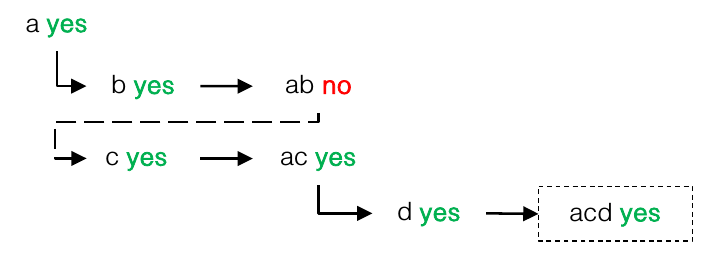
\includegraphics[scale=0.3]{Figures/iterator.png} 
\caption{Example of $^3$Cat-1 local scheduler prioritization heuristics}
\label{fig_heuristics}
\end{figure}

\item \textbf{Task definition}: Task objects contain all the relevant parameters and information for the scheduler. Each task is described with a task identifier, the task priority, and the restrictions for temperature, radiation or position domains. Finally, apart from providing the periodicity and the initial delay, the duration of a task is also defined.  Periodic tasks that should only be scheduled a given number of times, can provide the number of iterations.

\end{enumerate}

Some of these characteristics have to be adapted for the Local-Global context and extended functionalities needed to actually have a practical \emph{Local} entity have to be added. These changes are described below:

\begin{enumerate}
\item \textbf{Calculate $\Delta_i$ scheduling solutions.} Simply repeating the execution of the task scheduler $\Delta_i$ times is not sufficient and neither it is time nor memory efficient. Moreover, it will give $\Delta_i$ identical solutions. The solver must be forced to iterate $\Delta_i$ times for exploring the solutions space and collect a number of them.

The main trouble here is to avoid identical solutions, but the solution is in the core of Prolog's logic: as it is a declarative programming language, its execution procedure is based on checking that the input query can be proven as true according to the input facts and rules that constrain and define the problem. Whenever during the execution of the query an inconsistency is found, backtracking is used to a previous state and explores other possible conditions that are able to satisfy that inconsistency. In this case, this built-in backtracking capabilities could be used to find more than one scheduling solution that satisfies all the constrain.

\item \textbf{Enabling solutions with ``unscheduled'' tasks.} %This iteration process generates a valid combination of tasks by gradually expanding an initial sub-problem with more tasks. It starts with the simplest sub-problem (e.g., ``allocate resources to task $a_1$'') and continuous adding subsequent tasks, backtracking in the combinations tree whenever an unfeasible problem is found.
At the moment, task priorities are not considered for the Local-Global policy. Hence the $^3$Cat-1 \emph{iterator} previously described is not needed. However, without this \emph{iterator} the core solver of this Prolog-based local scheduler is not able to provide a scheduling solution whenever a task set is unfeasible in the given time $T_w$.

The solution to this issue was to expand the scheduling time in such a way that an artificial extra period of time is added to the initial scheduling window. This period of time is special because it has \emph{infinite} resources, so any task can be scheduled within this time. Therefore, whenever a task or a number of them that cannot be scheduled because of resource or time constraints is found, the solver will simply provide a solution with these tasks placed in this extra time period.

\item \textbf{Figure of merit ($F$) definition and calculation.} A main part of the Local-Global policy is the figure of merit, which describes the goodness of each sub-solution reported to the \emph{Global} layer. A critical contribution of this thesis has been a proposal for the definition of $F$. This does not mean only to enumerate a set of variables that can describe the solution, but to study these variables and stablish a valid bounded adaptive combination of all of them depending on each parameter's contribution to the schedule. 

The figure of merit is the sole parameter of goodness information about each sub-solution that the \emph{Global} layer will receive. So, it is the unique information it has to obtain the optimal combination of sub-solutions. Instead of having an extensive knowledge of the resources available in each satellite, it only possesses the figure of merit's value. Because of that, the definition must be as complete as possible, containing all and only the variables that really characterize the sub-solution against any other one. $F$ is completely defined in section \ref{sec_F_LG}.

\item \textbf{Communication with the \emph{Global}.} The local scheduler has been designed to output the first found solution, but the \emph{Local} entity hast to send a set of sub-solutions to the \emph{Global} layer. %As it has been already said, the information that the \emph{Local} must transmit is limited to the subset of tasks included in each sub-solution, and its figure of merit.
For the version implemented in this thesis this communication with the \emph{Global} has been modelled as outputting to a file the $\Delta_i$ solutions found. This files generated by all the \emph{Local} schedulers will be later processed by the \emph{Global} process.

\end{enumerate}

Apart from these added abilities, the $^3$Cat-1 local scheduler was entirely revised and individually tested for ensuring the best performance.

\subsubsection{Formal Local-Global problem description}
\label{sec_F_LG}

The definition of the figure of merit $F$ is essential in the Local-Global policy, as it provides the \emph{goodness} of the global solution.

Let all the terms in the multiple-satellite multiple-task scheduling problem be defined:

\begin{description}
\item[$S$] Number of satellites in the constellation.
\item[$\Delta_i$] Golden number: number of sub-solutions requested to/delivered by satellite $i$. This value is either set dynamically by the global algorithm or generated statically to equalize the computational load in each local scheduler.
\item[$P_{ij}$] The set of sub-solutions generated by satellite $i$ to a given scheduling problem. This term is defined with the pair $\left\langle A_{ij}, F_{ij}\right\rangle$, where
\begin{description}
\item[$A_{ij}$] is the task subset\footnote{Letter $A$ is chosen to prevent confusing the term with time-related variables, denoted with $T$.} included in sub-solution $j$ of satellite $i$ and
\item[$F_{ij}$] is the figure of merit for sub-solution $j$ from satellite $i$.
\end{description}
\item[$T_\mathrm{begin}$] Absolute time at which the scheduling window begins. 
\item[$T_\mathrm{end}$] Absolute time at which the scheduling window ends.
\item[$T_w$] Scheduling time window shared across all satellites, defined as:
\begin{equation}
T_w = T_\text{end} - T_\text{begin}
\end{equation}
\end{description}

Five variables finally form the definition of the figure of merit $F$ value: deadline-based priority, resource utilization, eagerness, satellite processing utilization and responsiveness. This parameters are described below.

Since the Local-Global policy is aimed at planning tasks within the scheduling window $T_w$, the algorithm may yield a final combination of sub-solutions which excludes some tasks. This may be caused either due to their execution domains not being within the current $T_w$ (e.g., a point in the orbit which is never reached by any of the satellites in the constellation) or because the tasks are only present in sub-solutions that are not part of the final global one. In order to deal with this behaviour and to include a prioritization method for tasks with shorter deadlines, the global scheduler will consider a fixed number of future scheduling windows and will promote those solutions where there is a task with sorter deadline\footnote{Deadlines are time values set by ground operators corresponding to the task's $t_{\text{max}}^{a_j}$ value} than that. In order to formulate this feature, let the following terms be defined:
\begin{description}%[leftmargin=1.5cm,labelindent=!]
\item[$L_{ij}$] The minimum distance (in time) between a task deadline and $T_\text{begin}$, for sub-solution $j$ in satellite $i$. 
\item[$N_s$] Number of periods in deadline prioritization. $N_s$ is a static parameter (see (\ref{eq_local-global_deadline_def})). 
\end{description}

Therefore, the \textbf{prioritization term} $\mathbf{D_{ij}}$ can be defined as follows:
\begin{equation}
\label{eq_local-global_deadline_def}
D_{ij} = 
\begin{cases}
2-\dfrac{L_{ij}}{N_s \cdot T_w} & \text{if} \quad L_{ij} \leq N_s \cdot T_w\\
1 & \text{otherwise}
\end{cases}
\end{equation}

Despite the \emph{Global} section of the policy not requiring details about the resources and their capacity allocation to tasks (this is actually what \emph{Local} entities solve), part of a solution's figure of merit ($F_{ij}$), which represents the goodness of a solution, is computed from each satellite's resource usage that derives from each local plan. In order to complete $F$ definition, the capacities and consumptions of each (local) resource are defined:

\begin{description}
\item[$R_i$] Set of resources present in satellite $i$. Therefore, $\bigcup_i{R_i}$ represents the total set of resources of the infrastructure.
\item[$c_{ijk}(t)$] Aggregated\footnote{The sum of resource consumptions by each scheduled task.} consumption of resource $k$ for satellite $i$ and sub-solution $j$ at time $t$.
\item[$m_{ik}(t)$] Capacity of the resource $k$ for satellite $i$ at time $t$.
\end{description}

$\mathbf{C_{ij}}$ is then defined to provide a metric to evaluate sub-solutions in terms of \textbf{resource utilization} as:

\begin{equation}
C_{ij} = \max_{t}\left\lbrace \sum_{k \in R_i}\left(1-\dfrac{c_{ijk}(t)}{m_{ik}(t)}\right)\dfrac{1}{|R_i|}\right\rbrace \qquad C_{ij} \in \left[0,1\right]
\end{equation}

Another variable to evaluate the goodness of a given sub-solution is $\mathbf{G_{ij}}$, which somehow represents the \textbf{eagerness} of the local satellite $i$ with respect to the execution of tasks in sub-solution $j$. A sub-solution will be better if it includes more tasks. However, not all satellites are able to perform every task. Some tasks might have constraints that are impossible to meet for satellites (e.g., a position in the orbit that they never reach) or require the use of specialized instruments which are not common for all satellites. Therefore, the figure of merit needs to evaluate the goodness of a sub-solution with respect to the tasks which each satellite has the capability to execute. In order to do so, $G_{ij}$ is defined as follows:
\begin{description}
\item[$A'_i$] Subset of tasks that satellite $i$ has the capability to perform. If a given satellite is equipped with a resource $k$, but this resource does not have enough capacity to perform a given task, this task will still be present in this subset ($a \in A_i'$).
\end{description}

\begin{equation}
G_{ij} = \dfrac{|A_{ij}|}{|A'_i|}
\end{equation}

Having $G$ and $C$ to evaluate the the number of tasks in a sub-solution and the utilization of resources and $D$ to modify the figure of merit of priority tasks, the following parameters will assess the goodness of a sub-solution with respect to the satellite \textbf{utilization} ($\mathbf{U_{ij}}$) and \textbf{responsiveness} ($\mathbf{E_{ij}}$). 

\begin{eqnarray}
U_{ij} &=& \dfrac{t_{1(ij)}}{T_\text{end}}\\
E_{ij} &=& \dfrac{t_{1(ij)}-t_{0(ij)}}{T_w}
\end{eqnarray}

Where

\begin{description}
\item[$t_0$] Minimum start time among all tasks in sub-solution $j$, corresponding to $\min_{\forall a \in A_i'}{start(a)}$.
\item[$t_1$] Maximum end time among all tasks in sub-solution $j$, corresponding to $\max_{\forall a \in A_i'}{end(a)}$.
\end{description}

These five parameters describe in very different contexts the quality of the sub-solution, providing knowledge of each \emph{Local} entity to the \emph{Global} with small overhead. It should be observed that 	all the parameters are bounded within the interval $\left[0,1\right]$, with the exception of $D_{ij}$, which is bounded within the interval $\left[1,2\right]$. This could be unnecessary as long as every parameter was proportional to the goodness aspect it represents, but is required by the \emph{Global} entity to allow for an efficient optimization. Moreover, this bounding happens to give each parameter a range of values that can vary at most exactly a value equal to $1$, so the relative importance given to each parameter is normalized.

Putting everything together, the \textbf{figure of merit} $\mathbf{F}$ is finally defined as:
\begin{equation}
\label{eq_F_weighted}
F_{ij} = w_c\cdot C_{ij} + w_g\cdot G_{ij} + w_u\cdot U_{ij} + w_e\cdot E_{ij} + w_d\cdot D_{ij} 
\end{equation}

The combination of the five parameters is a weighted sum of their values, Where $w$ are the static weights for each parameter, which can modify the by-default balanced relative importance of each parameter.

%-----------------------------------
%	SUBSECTION 2
%-----------------------------------

\subsection{The Global algorithm}
\label{sec_LG_optimizations}
%Como ya se ha comentado, la capa global es un problema NP-hard de optimización. Complejidad en función de las variables que entran en juego (de forma simple).
%Desarrollo de un algoritmo eficiente: funcionamiento (ordered_list, cuándo cortamos la búsqueda...) gráficas.
%Coordinación con el local.
%Comparación de los tiempos de ejecución para un set aleatorio de sub-soluciones con un algoritmo de fuerza bruta ¡No! Eso va en resultados.

The global scheduling algorithm is basically a combinatorial optimization problem, that can be described as in (\ref{eq_local-global_global_optimization}). The \emph{Global} layer receives sub-solution sets of size $\Delta_i$. Each solution is described by the pair formed by the scheduled tasks set and its figure of merit $\left\langle A_{ij}, F_{ij}\right\rangle$. A potential solution is a combination of at most $S$ sub-solutions, selecting one or none for each satellite. However, it is very important to determine how the combination of sub-solutions can be qualified in terms of the figures of merit of each one of them.

Tthe values could simply be aggregated by summing them, but there is something that must be considered when combining scheduling sub-solutions: a task can appear in more than one sub-solution of the set forming the combination: how does this affect to the quality of this combination as a possible final global solution?

To reflect this degradation in the quality of the global solution, the sum of the $F$ values will be weighted with a multiplying factor that depends on the sum of the number of occurrences of all tasks ($N_b$) normalized to the maximum number of occurrences, which is equal to $S\cdot |A|$, where $S$ is the number of satellites in the constellation and $|A|$ is the number of input tasks. Below the complete definition of the global problem can be found, where the binary decision variables $x_{ij}=1$ if sub-solution $P_{ij}$ is part of the final combination and $0$ otherwise: 

\begin{subequations}
\label{eq_local-global_global_optimization}
\begin{align}
\text{Maximize} \qquad r(P) &= \left(\sum_{i=0}^{S-1}\sum_{j=0}^{\Delta_i-1}x_{ij}{\prod_{f \in F_{ij}}f}\right)\cdot\left(1-\dfrac{N_b}{S\cdot |A|}\right)\\
\text{where:} \qquad N_b &= \sum_{i=0}^{S-1}\sum_{j=0}^{\Delta_i-1}\sum_{k \in A}{B_{ijk}\cdot x_{ij}}\\
B_{ijk} &= \begin{cases}1 & \text{if} ~k \in A_{ij}\\ 0 & \text{otherwise}\end{cases}
\end{align}
\end{subequations}

The description of the \emph{Global} entity implementation is divided in three different subsections: the first one is devoted to briefly analyse the computational complexity of the optimization combinatorial problem to be solved, the second is basically an enumeration of the efficiency-oriented design and recursive improvements made on the algorithm, and finally in the third part the coordination with the \emph{Local} entity is explored. 

\subsubsection{Complexity analysis: an exploding combinatorial problem}

The optimization problem described in (\ref{eq_local-global_global_optimization}) is basically an optimal search problem characterised by mainly three variables: number of satellites $S$, number of sub-solutions provided by each satellite $\Delta$ and the number of scheduling input tasks $|A|$. The entire space of possible combinations is formed by combinations of $S$ elements in which each element is the sub-solution identity selected on each satellite. For instance, for a satellite constellation formed by 5 satellites and having that the first satellite provides 4 sub-solutions, the second provides 3, the third only 2, and both the fourth and the fifth provide 5 sub-solutions, a possible \emph{Global} combination can be represented as (see also Fig. \ref{fig_comb_repr}):

\begin{center}
$ \left(2 0 1 0 3\right) $
\end{center}

This would mean that this particular combination has selected the second sub-solution provided by the first satellite, the first sub-solution provided by the third and the third one from the fifth satellite. Note that it has not selected any sub-solution for the satellites 2 and 4.

\begin{figure}[h!]
\centering
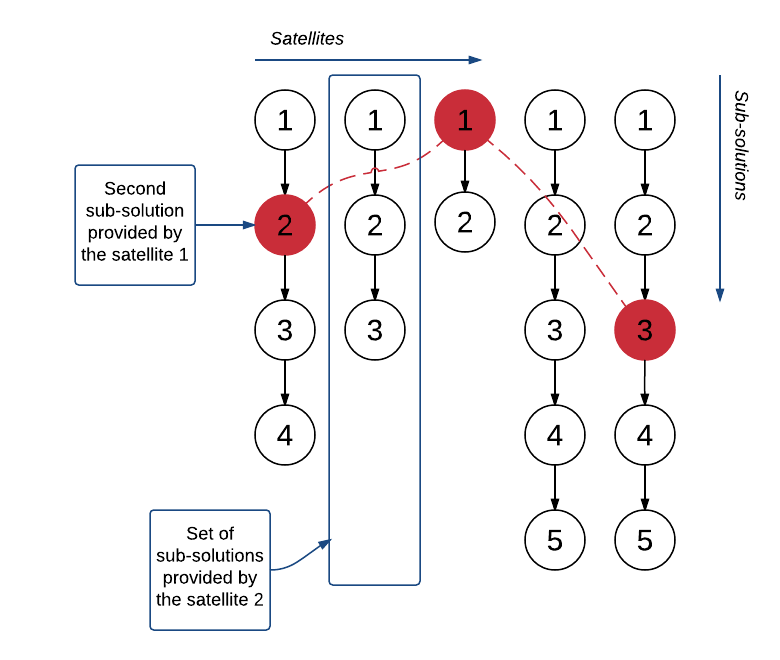
\includegraphics[scale=0.5]{Figures/comb_repr.png} 
\caption{A graphical representation of the combination of several sub-solutions}
\label{fig_comb_repr}
\end{figure}

Summarizing, it can be easily observed that the entire space of combinations would contain $\prod_{i=1}^{S}{\left(\Delta_i + 1\right)}$ combinations, where, for an homogeneous case where $\Delta_i = \Delta_{\text{system}}$, could be approximated to $\Delta_{\text{system}}^S$.

However, this expression does not completely include the complexity of the search. To find out the optimal combination the value of the $r(P)$ function should be calculated for each sub-solution combination, and this calculation depends basically on both the number of input tasks and the number of satellites of the system. This dependence is linear, as one can easily observe that the calculation is fully dominated by the sum of $F$ values, which varies linearly with $S$ (at most exactly $S$ sums must be done) and by the calculation of $N_b$, which depends linearly with the number of tasks $|A|$ (see (\ref{eq_local-global_global_optimization})).

In a basic computational complexity analysis notation, this would lead to a problem dependence on these three variables as shown below:

\begin{equation}
\label{eq_LG_complexity}
Global(\Delta_{\text{system}},S,|A|) \in \Theta\big((\Delta_{\text{system}})^S \cdot  |A|\big)
\end{equation}

\indent To conclude, it can be observed the evolution of the computational complexity when varying only one input with the others kept as a constant value:

\begin{itemize}
\item[--] If both $S$ and $|A|$ are kept constant a \textbf{potential variation} is observed.
\begin{equation}
Global(\Delta,S=S_0,|A|=|A|_0) \in \Theta\big(|A|_0(\Delta_{\text{system}})^{S_0}\big)=\Theta\big((\Delta_{\text{system}})^{S_0}\big)
\end{equation}

\item[--] If $\Delta_{\text{system}}=\Delta_0$ and $|A|$ is kept constant an \textbf{exponential variation} is observed.
\begin{equation}
Global(\Delta_{\text{system}}=\Delta_0,S,|A|=|A|_0) \in \Theta\big(|A|_0(\Delta_0)^S\big)=\Theta\big((\Delta_0)^S\big)
\end{equation}

\item[--] If $\Delta_{\text{system}}=\Delta_0$ and $S$ is kept constant a \textbf{linear variation} is observed.
\begin{equation}
Global(\Delta_{\text{system}}=\Delta_0,S=S_0,|A|) \in \Theta\big(|A|(\Delta_{\text{system}})^{S_0}\big)=\Theta(|A|)
\end{equation}

\end{itemize}

Therefore, an exponentially exploding problem is found when solving the \emph{Global} entity combinatorial optimization.

\subsubsection{An efficiency-oriented design of the combinatorial search}

The most basic and simple solution to this problem would be a brute force approach: exploring the entire space of possible combinations and simply comparing the values of the $r(P)$ function for each of them to finally select the one which maximizes it. However, when facing a problem that depends exponentially as the number of satellites and the $\Delta$ value for each one are increased, the brute force approach can be completely unfeasible.

That is why some efficient improvements have been applied and a careful study on the algorithmics and data structures that could be used has been performed.

To begin with, it is very important to observe two characteristics of the function to be optimized, $r(P)$ (see (\ref{eq_local-global_global_optimization})):
\begin{itemize}
\item It is a bounded function, concretely in the interval $\left[0, W\right]$, where $W$ is the sum of the $F$ weights (see (\ref{eq_F_weighted})): $w_c + w_g + w_u + w_e + w_d\cdot 2$ (remember that $D_{ij}$ is bounded in $\left[1, 2\right]$ instead of $\left[0, 1\right]$).
\item It is formed by the multiplication of two different terms: the sum of $F$ and a weighting value depending on the tasks occurrences, which is also bounded in $\left[0, 1\right]$
\end{itemize}

This means that $r(P)$ itself is bounded in the interval $\left[0, W\right]$ and, what is even more specific, in the interval $\left[1, \mathbb{F}\right]$, where $\mathbb{F}$ is the sum of $F$ of a particular combination.

Therefore, \textbf{finding out the way of exploring the space of combinations in a way that $\mathbb{F}$ value is decreasing, will allow to cut the exploration} as soon as a combination such that its $r(P)$ value is equal to its $\mathbb{F}$ value\footnote{This combination will be proved later to be the optimal combination.}, or a combination which $\mathbb{F}$ value is equal or below the maximum $r(P)$ found till now, is found.

A brief justification of these two affirmations is the one that follows: the fact that $r(P)$ value is bounded in the interval $\left[1, \mathbb{F}\right]$, and that the combinations space is being explored in decreasing $\mathbb{F}$ makes that no combination with lower $\mathbb{F}$ than any other with $r(P) = \mathbb{F}$ will have an $r(P)$ higher than this one because $r(P)$ is never greater than $\mathbb{F}$ (first cutting context) and that no combination with lower $\mathbb{F}$ than the maximum $r(P)$ value found till now will have a higher $r(P)$ than this maximum, for the same reason (second cutting context). In Fig. \ref{fig_r_vs_F} an example of this early searching cut can be seen.

\begin{figure}[h!]
\centering
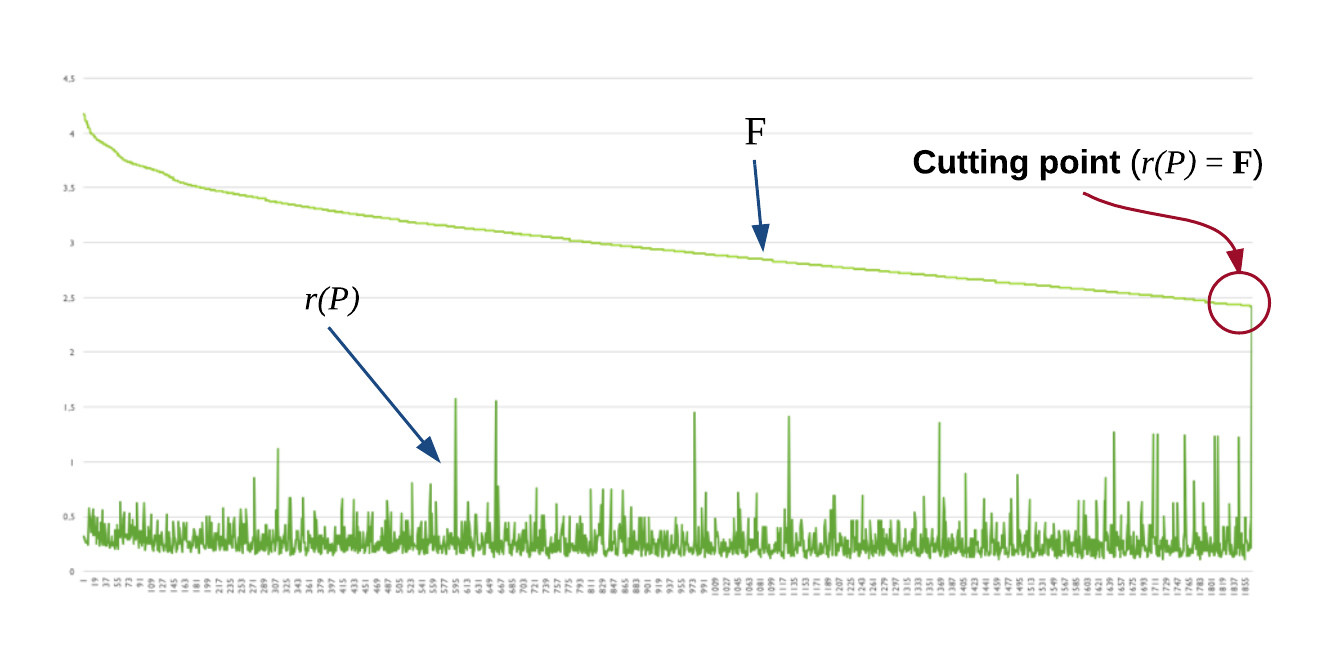
\includegraphics[width=\linewidth]{Figures/r_vs_F.png} 
\caption{Efficient optimal combination search}
\label{fig_r_vs_F}
\end{figure}

The search heuristics designed and implemented to enable a way of exploring the combinations space in decreasing $\mathbb{F}$ is completely explained in Appendix \ref{AppendixB}. In this project, this optimized design has been programmed using C language, and an efficient ordered list library has been also developed in order to have everything in the code controlled for best performance. In chapter \ref{Chapter4}, Fig. \ref{fig_global_brute}, particular results for this implementation compared with a brute force search are shown.

\subsubsection{Coordination with the \emph{Local} entities}

Concluding this section, this part will be devoted to explain the implementation of the \emph{Global}'s process which is in charge of collecting all the solutions submitted by all the \emph{Local} entities and process them for preparing the optimization search described before.

In the simulations performed in this work, the \emph{Local} entities write out in a text file the $\Delta_i$ sub-solutions, detailing for each one the subset of tasks included and the $F$ value.

Therefore, the \emph{Global} has to read that output text files and process them to initialize the internal variables that will represent the satellites' sub-solutions for combining them. If any of the satellites has not been able to send its sub-solutions (e.g., it is down or is not able to communicate with the \emph{Global} entity), the process simply considers it as it had a $\Delta_i = 0$.

At last, this input processing instance orders by descending $F$ value each set of sub-solutions, as the optimized combinatorial search requires.

%----------------------------------------------------------------------------------------
%	SECTION 2
%----------------------------------------------------------------------------------------

\section{Price-based algorithm implementation}
\label{sec_MBimplementation}

In order to implement the algorithm described in \cite{Edalat09}, some implementation details which are not included in the paper (e.g., the system architecture, the communication cost, the scheduling time window...) have been designed. Also some other aspects of the algorithm, such as the price calculation or some synchronization problems, have been improved for a best performance in the tests again the Local-Global policy. In this section the main features of this implementation are described, while in Appendix \ref{AppendixA} all the modifications over the original proposal are detailed.

%-----------------------------------
%	SUBSECTION 1
%-----------------------------------
\subsection{A state graph model}
%Describir el sistema según un grafo de estados.
%Implementación en Erlang, comunicación "real" entre nodos, arquitectura líder-esclavos.
%Ventana de tiempo concreta
%Nada de Listing Phase: sistema simple de dependencias
%Variables que mantiene cada nodo: Communication Cost como distancia entre satélites

A good approach for implementing a distributed algorithm like this is to model each node in the system as a state graph. In this way, programming the nodes is limited to programming all the possible states in the node, the state changes whenever it arrives to the system a particular message (or any other particular event occurs) with the functionalities performed in any of these states and the variables maintained by the node.

In this case, all the \emph{sellers} can be in two different states: WAITING and LISTENING. In the first one, the satellite is ready to begin a scheduling process as soon as a TASK message arrives to the system. In the second state, the system is performing a scheduling process and the node is waiting to transmit its task bid or surrender if a lower-price bid is received from other satellite. The flowchart of the implemented algorithm can be seen in Fig. \ref{fig_state_graph}.

\begin{figure}[h!]
\centering
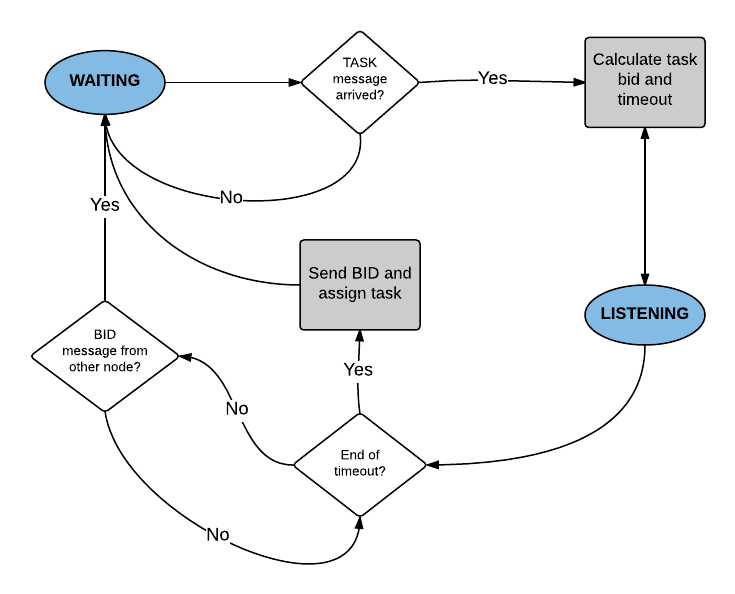
\includegraphics[scale=0.7]{Figures/flow_mb.png} 
\caption{Price-based policy flowchart}
\label{fig_state_graph}
\end{figure}

The auxiliary functionalities that have been implemented are mainly two: the price calculation and the task addition to the local scheduler. The first one is a calculation based on the current state of the node and the second is executed whenever the node has won a scheduling process and assigns itself the task, reserving the corresponding resources and refreshing its own state knowledge.

The node's state knowledge will be now described. In this work the designed set of local variables maintained by each satellite are:

\begin{enumerate}
\item \textbf{Name.} The satellite's ID, used for identifying each satellite's message.
\item \textbf{Energy.} The amount of energy that has not been reserving for executing already assigned tasks.
\item \textbf{Processor release time.} The time instant in which the processor will finish the current scheduled tasks.
\item \textbf{Beginning time.} The initial time of the current scheduling window, used for determining timestamps relative to it, for optimizing the overhead caused by the use of a long absolute time stamp.
\item \textbf{Peers list.} The other satellites' IDs present in the constellation. It also includes the communication cost for each one.
\item \textbf{Schedule.} The local schedule assigned until that particular moment, generated from the different scheduling processes that have been completed since the beginning of the scheduling window.
\item \textbf{Task assignment.} For each already assigned tasks, it contains the ID of the satellite that has been assigned to execute it.
\end{enumerate}

The current implementation has been developed in Erlang code, a functional programming and distributed systems-oriented language. Its distributed nature has allowed to directly simulate different nodes and a real message passing system between the nodes. This truly distributed environment has required a specific architecture design for a better system management.

Because of that, a \emph{leader-slaves} centralized architecture has been implemented. The \emph{leader-slave} relationship is only valid for system registering or de-registering\footnote{Whenever a satellite wants to enter in the system, it has to communicate it to the current leader, and the same for whenever a satellite leaves the system.}, although it is meaningless for the scheduling algorithm.

Another feature of this implementation has been the simplification of the \emph{Listing Phase} (see section \ref{sec_MBdescription}). Instead of dividing complex tasks into simpler ones, an already dependence-processed input task sets has been considered. The dependence among two tasks has been modelled as an added task attribute which contains the ID of its \emph{predecessor} task i.e. the task that must be completed to begin this one. In the next section the task dependence's importance on calculating the task bid on a scheduling process is explained along with other implemented modifications in order to optimize the algorithm.